\documentclass{article}
\usepackage{tikz}
\usepackage{geometry}
\usepackage{amsmath}
\usepackage{array}
\usetikzlibrary{arrows.meta,positioning,shapes.geometric}
\geometry{margin=1in}

\title{Unified Implementation Plan for Autonomous CNC Toolpath System}
\author{M365 Copilot}
\date{\today}

\begin{document}
\maketitle

\section{Included Source Prompts}
\subsection{Toolpath Prompt}
\textit{You are a software+mechanical engineer tasked with generating a toolpath generation software... tool must enter from outside the face.}

\subsection{Feeds and Speeds Context}
\textit{You are selecting feeds and speeds based on material, tool, and operation with shop-floor adjustments.}

\subsection{Factory Simulation Prompt}
\textit{You are developing a simulation of an autonomous factory with multiple CNC machines, toolpaths, scheduling, and optimization policies.}

\section{System Architecture}

\begin{center}
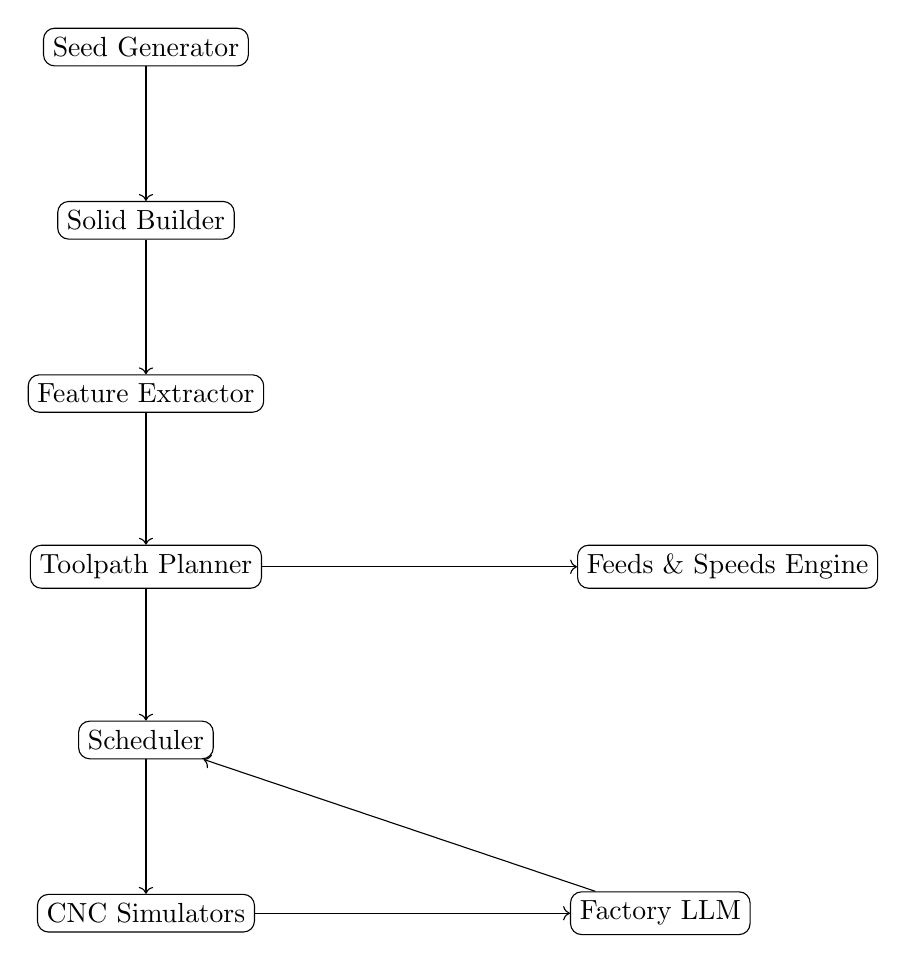
\begin{tikzpicture}[node distance=2.2cm, every node/.style={draw, rectangle, rounded corners, align=center}]

\node (seed) {Seed Generator};
\node (solid) [below of=seed] {Solid Builder};
\node (features) [below of=solid] {Feature Extractor};
\node (planner) [below of=features] {Toolpath Planner};
\node (fs) [right=4cm of planner] {Feeds \& Speeds Engine};
\node (scheduler) [below of=planner] {Scheduler};
\node (machines) [below of=scheduler] {CNC Simulators};
\node (factory) [right=4cm of machines] {Factory LLM};

\draw[->] (seed) -- (solid);
\draw[->] (solid) -- (features);
\draw[->] (features) -- (planner);
\draw[->] (planner) -- (scheduler);
\draw[->] (scheduler) -- (machines);
\draw[->] (planner) -- (fs);
\draw[->] (machines) -- (factory);
\draw[->] (factory) -- (scheduler);

\end{tikzpicture}
\end{center}

\section{Implementation Modules}

\subsection{1. Solid Builder}
- Generate 1--4 cuboids (axis-aligned) \\
- Add pockets and holes \\
- Output: face list with wall/cliff metadata

\subsection{2. Feature Extractor}
- Identify top faces $P_i$ \\
- Label edges: Wall / Cliff / Level

\subsection{3. Toolpath Planner}
Core algorithm: \\
- Classify edges (wall, cliff) \cite{toolpath} \\
- Compute safe region $S_i = P_i \ominus B_{blocked}$ \cite{toolpath} \\
- Generate raster paths \\
- Ensure entry from safe edge

\subsection{4. Feeds \& Speeds Engine}
- Compute RPM from cutting speed \cite{feeds} \\
- Compute feed: $F = N Z f_z$ \cite{feeds} \\
- Adjust based on chatter, rigidity

\subsection{5. Drilling \& Entry Module}
- Peck drilling rules (0.25D--1D) \cite{feeds} \\
- Entry selection (plunge, ramp, helix)

\subsection{6. Scheduler}
- Assign parts to machines \\
- Optimize based on policy:
\begin{itemize}
\item Min time
\item Max tool life
\item Min cost
\item Best finish
\end{itemize}

\subsection{7. CNC Simulator}
- Execute G-code \\
- Track:
\begin{itemize}
\item Tool wear
\item Time
\item Errors
\end{itemize}

\section{Algorithm Pipeline}
\begin{verbatim}
seed -> build geometry -> extract features
-> generate toolpath -> assign feeds/speeds
-> schedule -> simulate -> feedback
\end{verbatim}

\section{Key Data Structures}
\begin{itemize}
\item Face: polygon + height + edges
\item Tool: diameter, life, cost
\item Machine: queue, tool crib
\item Feature: pocket, hole, face
\end{itemize}

\section{Weaknesses and Missing Information}

\subsection{Geometry Limitations}
- Only cuboids supported \\
- No curved surfaces or rotations

\subsection{Toolpath Gaps}
- No cutter deflection modeling \\
- No corner smoothing/blending

\subsection{Physics Gaps}
- No cutting force model \\
- No power/torque constraints

\subsection{Feeds \& Speeds Limitations}
- Empirical only (no adaptive control) \\
- Missing tool coating effects

\subsection{Simulation Gaps}
- Tool crib not fully implemented \\
- Error handling incomplete \\
- Multi-machine coordination unclear

\subsection{Optimization Gaps}
- Multi-objective optimization not formalized \\
- No global optimization across features

\subsection{Software Gaps}
- Dependency on outdated OCC environment \\
- No API contract between modules

\section{Recommended Improvements}
\begin{itemize}
\item Add force and power models
\item Implement adaptive feed control
\item Extend geometry kernel
\item Formalize API between modules
\item Add unit tests and benchmarking
\end{itemize}

\section{Hierarchical Error-Aware Multi-Agent Control System}

\subsection{Overview}
To address error handling and multi-machine coordination, we introduce a hierarchical control architecture enabling real-time anomaly interpretation, safe intervention, and coordinated mitigation across CNC agents and the factory system.

\subsection{Integrated Execution Loop}
The base loop:
\begin{center}
\texttt{simulate -> feedback}
\end{center}
is extended to:
\begin{center}
\texttt{simulate -> prompt -> transform -> CNC reasoning -> safety check -> escalate -> factory reasoning -> mitigate -> resume}
\end{center}

\subsection{8.2 Integrated Execution Loop (Component Definitions)}

The execution loop is:

\begin{center}
\texttt{
$\text{simulate} \rightarrow \text{prompt} \rightarrow \text{transform} \rightarrow \text{CNC reasoning} \rightarrow \text{safety check} \rightarrow \text{escalate} \rightarrow \text{factory reasoning} \rightarrow \text{mitigate} \rightarrow \text{resume}
$}
\end{center}

\begin{enumerate}
\item \textbf{Simulate} \
Advance machine and factory state by one control interval. This stage executes scheduled operations, updates tool wear, progresses jobs, and captures current telemetry (tick, machine status, queue depth, active tool, and error state).
\textit{Output:} Updated runtime state and raw operational signals.

\item \textbf{Prompt} \
Generate an event prompt when anomalous or decision-relevant conditions are detected (for example chatter, tool breakage risk, queue imbalance, or policy conflict). Prompts may originate from sensors, rules, or operator input.
\textit{Output:} Human-readable or structured trigger message.

\item \textbf{Transform} \
Convert prompt text and runtime context into a structured decision payload. This transformation standardizes fields such as event type, severity, affected machine, tool context, job context, and recent history.
\textit{Output:} Normalized context object for deterministic and LLM reasoning.

\item \textbf{CNC Reasoning} \
Perform local machine-level diagnosis and generate candidate actions (for example reduce feed, pause, replace tool, continue with caution). This stage prioritizes local constraints and machine safety boundaries.
\textit{Output:} Ranked local action candidates with rationale and confidence.

\item \textbf{Safety Check} \
Validate each candidate against hard safety rules and operational invariants. Unsafe candidates are rejected immediately. Safety-critical events may force immediate stop behavior.
\textit{Output:} Safety-filtered candidate set and risk labels (safe, risky, critical).

\item \textbf{Escalate} \
If local resolution is insufficient, high-risk, or has system-wide implications, escalate the case to factory-level coordination with full context package and local reasoning trace.
\textit{Output:} Escalation record linking machine context to factory-level decision flow.

\item \textbf{Factory Reasoning} \
Evaluate global tradeoffs across machines, queues, inventory, and policy objectives. Compute coordinated actions such as rerouting, policy tuning, maintenance sequencing, or controlled hot-swap proposals.
\textit{Output:} Factory-level mitigation plan with expected impact and rollback strategy.

\item \textbf{Mitigate} \
Execute approved corrective actions. For any hot-swap action, enforce mandatory human approval before execution. Log approval decision, action dispatch, and pre/post state snapshots for evaluation.
\textit{Output:} Applied mitigation commands, audit events, and verification checkpoints.

\item \textbf{Resume} \
Return machine and factory workflows to normal progression from a verified safe state. Monitor short-horizon outcomes to confirm resolution and trigger rollback if regression is detected.
\textit{Output:} Stable continuation of production with outcome metrics recorded.
\end{enumerate}

\paragraph{Operational Notes}
\begin{itemize}
\item Every transition emits telemetry events for replay and post-incident analysis.
\item Decision and outcome events are correlated for effectiveness scoring.
\item Human approval is a hard gate for all hot-swap operations before mitigation execution.
\end{itemize}



\subsection{Design Principles}
\begin{itemize}
\item Separation of concerns: CNC-local vs Factory-global
\item Structured context over raw prompt text
\item Safety-first execution boundaries
\item Human-in-the-loop supervision
\end{itemize}

\section{Expanded Query, Telemetry, and Human-Approved Hot-Swap Architecture}

\subsection{Problem Statement}
Current updates are concentrated in routing/policy/tool-optimization paths. The system needs:
\begin{itemize}
\item richer query support backed by runtime data,
\item persistent telemetry for decision context,
\item full action/event logs for post-event evaluation,
\item strict governance where every hot-swap requires explicit human approval.
\end{itemize}

\subsection{Mandatory Human Approval Rule}
\textbf{Rule:} No hot-swap may execute without explicit human approval. \\
This applies to:
\begin{itemize}
\item runtime strategy swaps (routing, policy, tool parameters),
\item plugin/module swaps (install, enable, disable, rollback).
\end{itemize}
Emergency stop/abort remains allowed without pre-approval because it is a safety control, not a hot-swap, but it must still be logged.

\subsection{Expanded Query Taxonomy}
\begin{itemize}
\item Observability queries: machine state, queue, tool crib, KPI.
\item Deterministic control actions: scheduling/policy/routing controls.
\item Advisory optimization actions: LLM + rule-based recommendations.
\item Safety/emergency actions: stop, abort, escalation.
\item Telemetry analytics queries: action effectiveness, trend analysis, incident replay.
\item Plugin lifecycle actions: install/enable/disable/rollback (approval-gated).
\end{itemize}

\subsection{Control Flow with Human Approval Gate}
\begin{center}
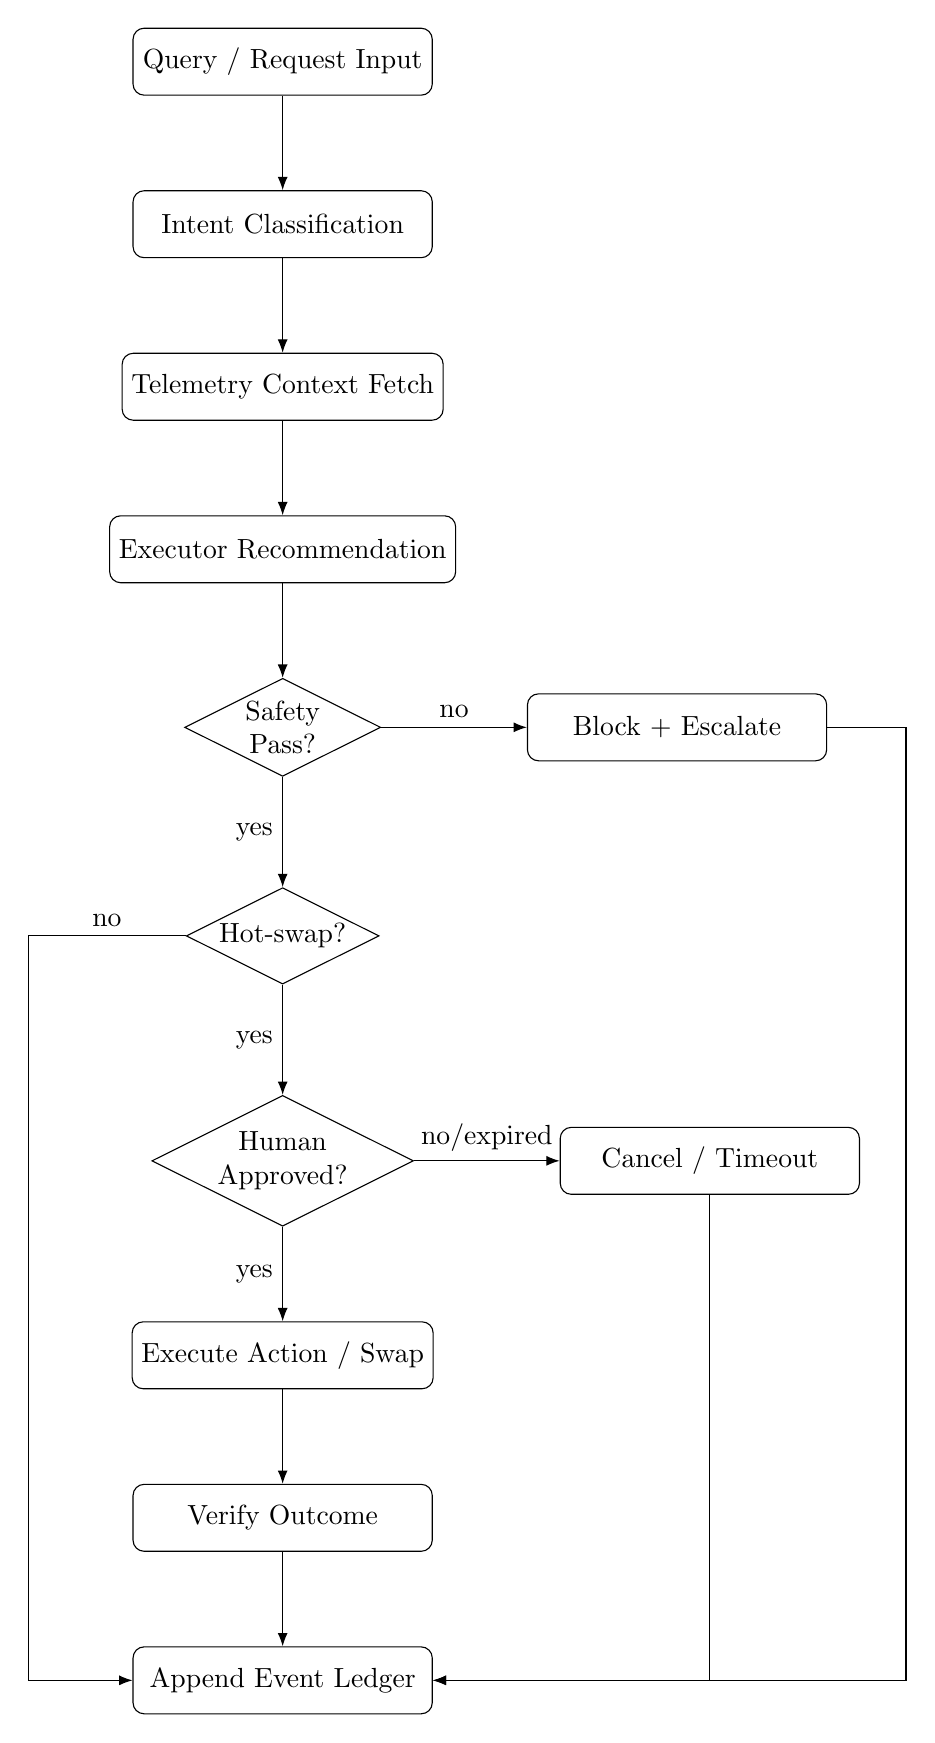
\begin{tikzpicture}[
node distance=1.20cm,
box/.style={draw, rounded corners, minimum width=3.8cm, minimum height=0.85cm, align=center},
decision/.style={draw, diamond, aspect=2, align=center, inner sep=1pt},
>=Latex
]
\node[box] (q) {Query / Request Input};
\node[box, below=of q] (classify) {Intent Classification};
\node[box, below=of classify] (ctx) {Telemetry Context Fetch};
\node[box, below=of ctx] (exec) {Executor Recommendation};
\node[decision, below=of exec] (safe) {Safety\\Pass?};
\node[decision, below=of safe, yshift=-0.2cm] (approval) {Hot-swap?};
\node[decision, below=of approval, yshift=-0.2cm] (human) {Human\\Approved?};
\node[box, below=of human] (apply) {Execute Action / Swap};
\node[box, below=of apply] (verify) {Verify Outcome};
\node[box, below=of verify] (log) {Append Event Ledger};

\node[box, right=1.85cm of safe] (halt) {Block + Escalate};
\node[box, right=1.85cm of human] (cancel) {Cancel / Timeout};

\draw[->] (q) -- (classify);
\draw[->] (classify) -- (ctx);
\draw[->] (ctx) -- (exec);
\draw[->] (exec) -- (safe);
\draw[->] (safe) -- node[left]{yes} (approval);
\draw[->] (safe.east) -- node[above]{no} (halt.west);
\draw[->] (approval.west) -- node[above]{no}++(-2cm,0) |- (log.west);
\draw[->] (approval) -- node[left]{yes} (human);
\draw[->] (human) -- node[left]{yes} (apply);
\draw[->] (human.east) -- node[above]{no/expired} (cancel.west);
\draw[->] (apply) -- (verify);
\draw[->] (verify) -- (log);
\draw[->] (halt.east) -- ++(1cm,0) |- (log.east);
\draw[->] (cancel) |- (log.east);
\end{tikzpicture}
\end{center}

\subsection{Data Collection and Query Supplementation Architecture}
\begin{center}
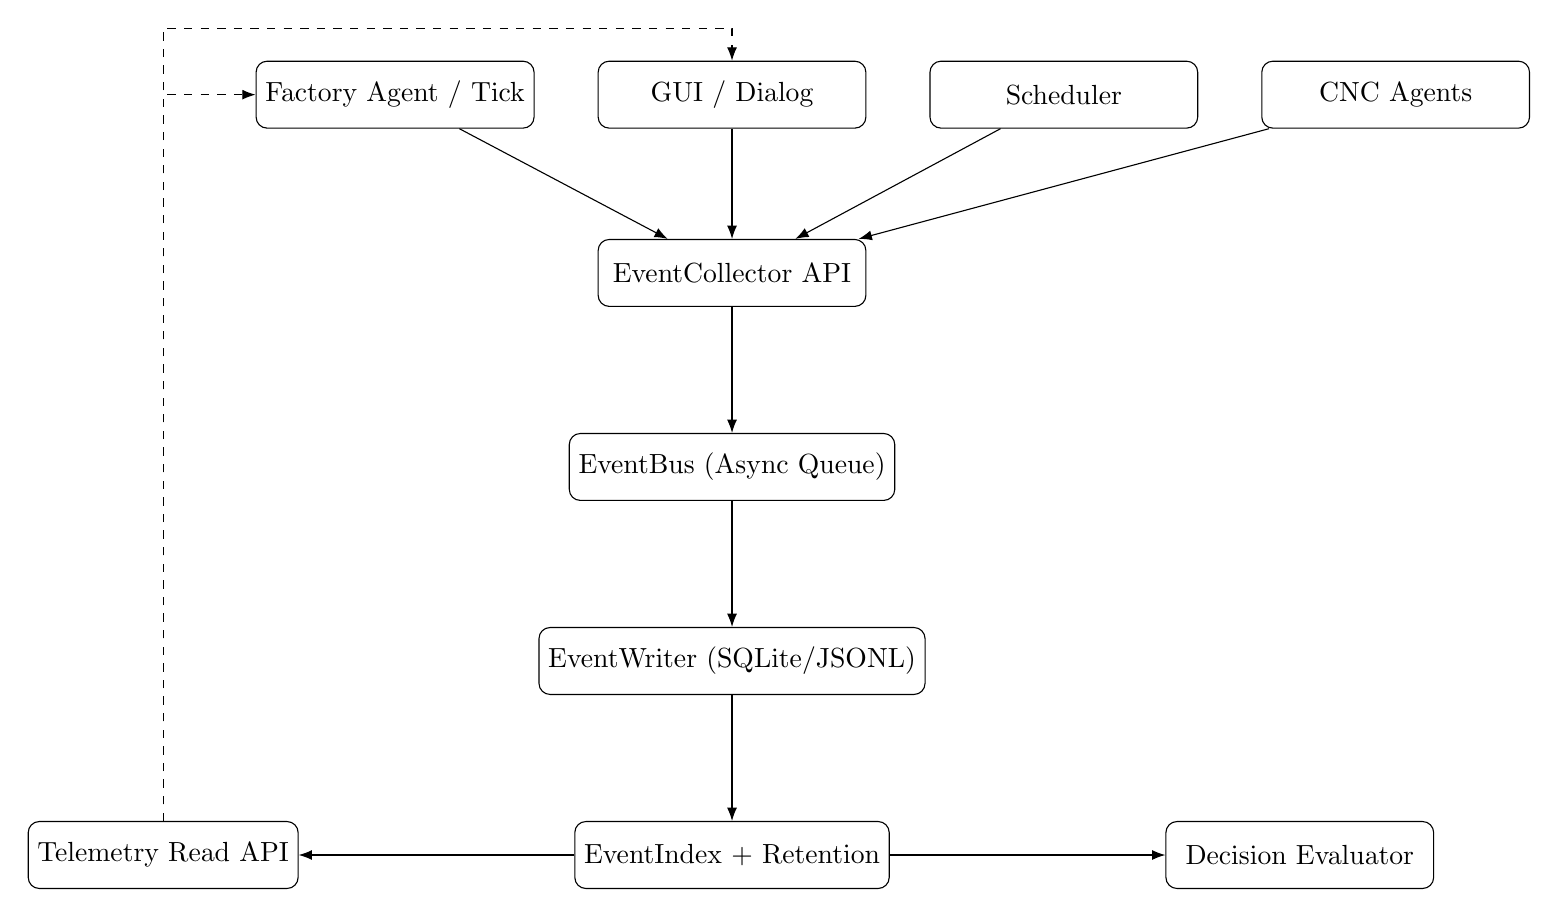
\begin{tikzpicture}[
node distance=1.6cm,
box/.style={draw, rounded corners, minimum width=3.4cm, minimum height=0.85cm, align=center},
>=Latex
]
\node[box] (p1) {Factory Agent / Tick};
\node[box, right=0.8cm of p1] (p2) {GUI / Dialog};
\node[box, right=0.8cm of p2] (p3) {Scheduler};
\node[box, right=0.8cm of p3] (p4) {CNC Agents};


\node[box, below=1.4cm of p2] (collector) {EventCollector API};
\node[box, below=of collector] (bus) {EventBus (Async Queue)};
\node[box, below=of bus] (writer) {EventWriter (SQLite/JSONL)};
\node[box, below=of writer] (index) {EventIndex + Retention};
\node[box, left=3.5cm of index] (readapi) {Telemetry Read API};
\node[box, right=3.5cm of index] (eval) {Decision Evaluator};

\draw[->] (p1) -- (collector);
\draw[->] (p2) -- (collector);
\draw[->] (p3) -- (collector);
\draw[->] (p4) -- (collector);
\draw[->] (collector) -- (bus);
\draw[->] (bus) -- (writer);
\draw[->] (writer) -- (index);
\draw[->] (index) -- (readapi);
\draw[->] (index) -- (eval);
\draw[->, dashed] (readapi) |- (p1);
\draw[->, dashed] (readapi) |- ++(0,10.5cm) -| (p2.north);
\end{tikzpicture}
\end{center}

\subsection{Unified Event Envelope}
Every event uses:
\begin{center}
\begin{tabular}{|>{\raggedright}p{5.0cm}|>{\raggedright\arraybackslash}p{9.0cm}|}
\hline
Field & Meaning \\
\hline
event\_id, event\_type & Unique id and canonical event category \\
\hline
tick, timestamp\_utc, wall\_time\_ms & Logical and wall-clock timing \\
\hline
machine\_id, job\_id, seed & Operational context \\
\hline
source, category, severity & Producer identity and severity class \\
\hline
correlation\_id, causation\_id & Cross-event lineage for replay \\
\hline
payload & Typed event-specific data \\
\hline
\end{tabular}
\end{center}

\subsection{Mandatory Hot-Swap and Approval Events}
\begin{itemize}
\item swap\_requested
\item swap\_risk\_assessed
\item swap\_approval\_requested
\item swap\_approved / swap\_rejected / approval\_expired
\item swap\_executed
\item swap\_verified
\item swap\_rolled\_back
\item override\_denied\_without\_approval
\end{itemize}

\subsection{Human Approval Invariants}
\[
\text{ExecuteHotSwap}(r) \Rightarrow \text{ValidApprovalToken}(r)
\]
\[
\text{ValidApprovalToken}(r) \Rightarrow
\left(
\text{scope\_match} \land \text{not\_expired} \land \text{approver\_present}
\right)
\]
\[
\neg \text{ValidApprovalToken}(r) \Rightarrow \text{SwapBlocked}(r)
\]

\subsection{Dual-Layer Hot-Swap Lifecycle (Approval-Gated)}
\begin{center}
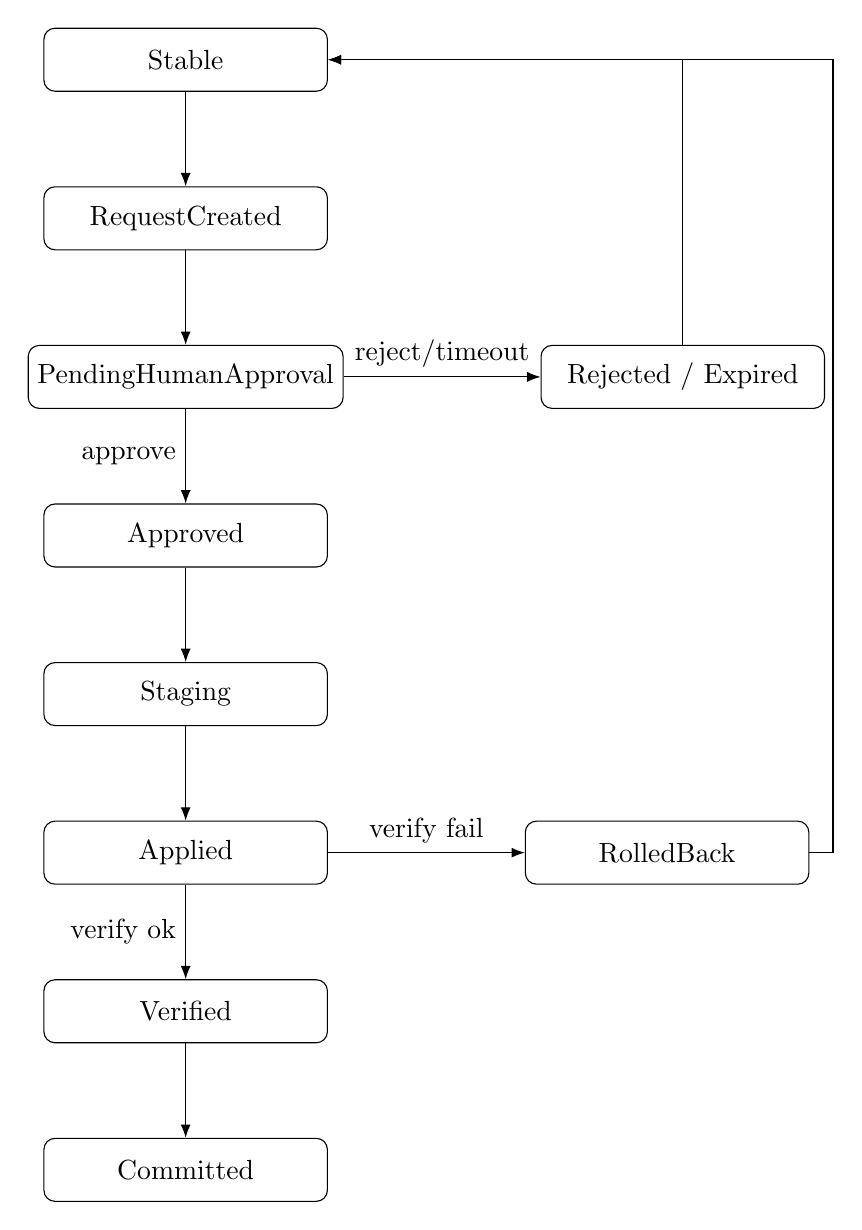
\begin{tikzpicture}[
node distance=1.2cm,
state/.style={draw, rounded corners, minimum width=3.6cm, minimum height=0.8cm, align=center},
>=Latex
]
\node[state] (stable) {Stable};
\node[state, below=of stable] (req) {RequestCreated};
\node[state, below=of req] (pending) {PendingHumanApproval};
\node[state, below=of pending] (approved) {Approved};
\node[state, below=of approved] (staging) {Staging};
\node[state, below=of staging] (applied) {Applied};
\node[state, below=of applied] (verified) {Verified};
\node[state, below=of verified] (committed) {Committed};

\node[state, right=2.5cm of pending] (rejected) {Rejected / Expired};
\node[state, right=2.5cm of applied] (rollback) {RolledBack};

\draw[->] (stable) -- (req);
\draw[->] (req) -- (pending);
\draw[->] (pending) -- node[left]{approve} (approved);
\draw[->] (approved) -- (staging);
\draw[->] (staging) -- (applied);
\draw[->] (applied) -- node[left]{verify ok} (verified);
\draw[->] (verified) -- (committed);
\draw[->] (pending.east) -- node[above]{reject/timeout} (rejected.west);
\draw[->] (applied.east) -- node[above]{verify fail} (rollback.west);
\draw[->] (rejected) |- (stable.east);
\draw[->] (rollback.east) -- ++(0.3cm,0)  |- (stable.east);
\end{tikzpicture}
\end{center}

\subsection{Action and Solution Evaluation}
Each decision is linked to action outcomes by correlation id and request id. Effectiveness is scored by:
\[
U = w_q \Delta q - w_t \Delta t - w_c \Delta c + w_r R
\]
where:
\begin{itemize}
\item $\Delta q$ is quality improvement,
\item $\Delta t$ is time increase,
\item $\Delta c$ is cost increase,
\item $R$ is resolution success indicator,
\item $w_q, w_t, w_c, w_r$ are policy weights.
\end{itemize}
Outcomes are classified as effective, neutral, or regressive.

\subsection{Storage, Indexing, and Retention}
\begin{itemize}
\item Append-only telemetry store (SQLite first, JSON payload field).
\item Core indexes: event\_type, tick, machine\_id+tick, job\_id, request\_id, timestamp\_utc.
\item Retention tiers: short-term high detail, long-term aggregated archives.
\item Redaction policy for sensitive operator text and model payloads.
\end{itemize}

\subsection{Phased Rollout}
\textbf{Phase A:} approval request model and token enforcement for all hot-swap endpoints. \\
\textbf{Phase B:} mandatory hot-swap lifecycle and approval audit events. \\
\textbf{Phase C:} persistent telemetry writer and indexed query APIs. \\
\textbf{Phase D:} decision-outcome evaluator and incident replay timeline. \\
\textbf{Phase E:} supervisor dashboards for pending approvals and outcome quality.

\subsection{Verification Matrix}
\begin{itemize}
\item Unit: token validation, expiry, scope match, event schema integrity.
\item Integration: prove swap blocked without approval.
\item Integration: approve, reject, timeout branches.
\item Replay: reconstruct request -> approval -> execution -> outcome chain.
\item Documentation: TeX compile and TikZ rendering checks.
\end{itemize}

\section{Conclusion}
This unified plan now combines geometry generation, toolpath planning, machining parameters, factory scheduling, telemetry-backed decision support, and strict human-governed hot-swap control. The architecture is designed for safe autonomy with explicit approval, full auditability, and measurable solution quality over time.

\end{document}